% Created 2012-04-29 Sun 19:01
\documentclass[a4paper,11pt]{scrartcl}
\usepackage[danish,british]{babel}
\usepackage[english]{varioref}
\usepackage{tohojo-xe}
\selectlanguage{british}
\usetikzlibrary{positioning,shadows,arrows}
\fancyfoot[OR,EL]{\footnotesize Page~\thepage~of~\pageref{LastPage}}

\title{Cased Based Reasoning System}
\author{Toke Høiland-Jørgensen}
\date{29 April 2012}
\hypersetup{
  pdfkeywords={},
  pdfsubject={},
  pdfcreator={Emacs Org-mode version 7.8.06}}

\begin{document}

\maketitle

\begin{center}
\sffamily
{\large COMPSCI 767 assignment 1}\\
Semester 1, 2012\\
University of Auckland
\end{center}

\setcounter{tocdepth}{3}
\tableofcontents
\vspace*{1cm}

\section{Introduction}
This report provides details on a case based reasoner implementation
for the travel case base. The first section of the report documents
the application design, including the case retrieval mechanism,
similarity metrics, adaptation mechanism, code structure and
interface. The second section provides information on installing and
running the application.

The code, if not found along with the report, can be obtained from
GitHub at \url{https://github.com/tohojo/cbr-system}.
\clearpage

\section{Application design}
This section details the overall design of the CBR system application.
This consists of five parts: retrieval of cases, similarity metrics,
adaptation, code structure and interface. Familiarity with CBR
concepts is assumed, and only notes relating to the specific
implementation are included.

\subsection{Case retrieval}
This section describes the case retrieval process in general terms.
For details of how this relates to the code, see the section on code
structure. The similarity metrics for the case base attributes are
explained in the next section on similarity metrics.

Retrieval is done using a simple $k$ nearest neighbour search, where a
submitted query is compared to each case in the case base to derive a
similarity for that case. Since the travel case base is quite small
(1470 cases), retrieval using this brute-force search method results
in sub-second query run performance, so a more efficient retrieval
algorithm is unnecessary.

After comparison, the cases are sorted by similarity in descending
order and the $k$ best matches are returned, where $k$ is
user-configurable and defaults to 2. Cases that have the same
similarity score for the current query are returned in arbitrary
order.

To derive a total similarity for a case, each attribute is compared to
the query attributes, and a weighed sum (with weights defined for each
attribute, see below) is calculated for the case. The normalised value
of this weighed sum is the case similarity.

Since a query need not include all attributes, only those attributes
included in the query are used for calculating the similarity metric.
This is different from the behaviour if a case in the case base is
missing an attribute\protect\footnote{No such cases exist in the
  travel case base, but in principle they might. } that is present in
the query: In this case a similarity of 0.0 is assumed for this
attribute.

\subsection{Similarity metrics}
Similarity metrics and weights are defined for each attribute of the
travel case base. In order to define similarity metrics, a
domain-specific interpretation of each attribute is necessary. This
section explains this interpretation and the resulting similarity
metrics and weights for each attribute. Similarity metrics are given
in the range $[0;1]$, and weights in the range $[1;\infty[$.

As a general note, because of the way matching works (i.e. absent
values from a query are ignored), the mere fact of an attribute being
present is evidence of a preference. I.e. some attributes (like
journey code or hotel name) do not make sense to specify in a query
unless there's a very strong preference of that exact value.

\subsubsection{Accommodation}
The accommodation attribute defines the quality of the holiday
accommodation. The possible values are either a holiday flat, or a one
to five star hotel. To simplify things, a holiday flat is interpreted
as a `zero-star' hotel. This means that matching can be done on the
number of stars (i.e. it turns into a linear match in the range 0-5).
Under the assumption that, all other things being equal, a better
accommodation type would be preferred, a `more is perfect' metric is
used for the comparison.

The type of accommodation is assumed to not be a defining attribute of
a holiday, and so to be of relatively low importance. Thus, it is
assigned the weight 2.

\subsubsection{Duration}
The duration of the holiday is measured in days. A simple numeric
distance is employed for the similarity metric. To normalise
distances, the range of possible durations is extracted from the case
base. Queries that fall outside this range is supported by dynamically
adjusting the range as appropriate.

It seems a fair assumption that a holiday can be straight-forwardly
modified to be longer, with a corresponding increase in price. Based
on this assumption, duration is an adjustable attribute (see the
section on adaptation for details on how this works). Because of this,
it is given a low weight of 1.

\subsubsection{Holiday type}
The holiday type is a type such as `Active', `Adventure', `City', etc.
of the holiday. The possible values for holiday types are entered
manually into a taxonomy tree. Matching is done by finding the closest
common ancestor of the values being compared. The value for that node
is the value of the similarity metric. The tree for holiday type is
taken from the example in the lecture
slides\footnote{\url{http://www.cs.auckland.ac.nz/~ian/CBR/cbr03.pdf}.}
and looks as follows (where the numbers in parenthesis is the
similarity when that node is the common ancestor):

\begin{center}
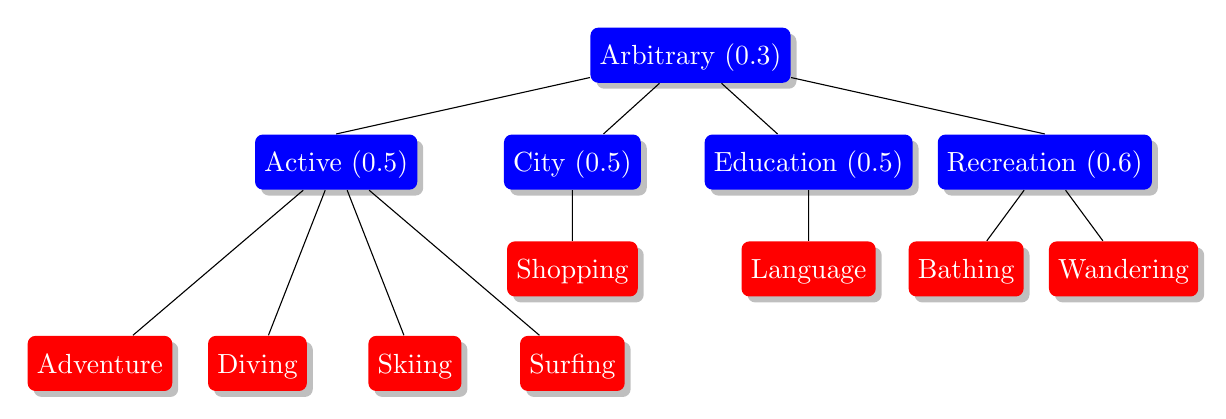
\begin{tikzpicture}[
every node/.style={rectangle, draw=none, rounded corners=1mm, fill=blue, drop shadow,
        align=center, text height=9pt, text depth=2pt, anchor=north, text=white, minimum height=7mm},
leaf/.style={fill=red},
level distance=1cm
]
  \node {Arbitrary (0.3)}[sibling distance=3cm]
      child { [sibling distance=2.0cm,level distance=2.2cm]
        node {Active (0.5)}
           child {node [leaf] {Adventure}}
           child {node [leaf] {Diving}}
           child {node [leaf] {Skiing}}
           child {node [leaf] {Surfing}}}
      child {
        node {City (0.5)}
          child {node [leaf] {Shopping}}}
      child {
        node {Education (0.5)}
          child {node [leaf] {Language}}}
      child { [sibling distance=2cm]
        node {Recreation (0.6)}
          child {node [leaf] {Bathing}}
          child {node [leaf] {Wandering}}}
      ;
\end{tikzpicture}
\end{center}

Considering that e.g. a skiing holiday is quite significantly
different from a shopping holiday, the type of holiday is considered
an important metric, and given a weight of 10.

\subsubsection{Hotel}
The hotel attribute is the name of the hotel for the holiday. Since
no valid characteristics can be extracted from the name of the hotel
itself (and the type of hotel is covered in its own attribute) a match
is made only on the exact name, and a match of zero otherwise. it is
assumed that if a hotel name is specified in the query, it is a very
outspoken preference to go to a specific hotel, and thus it is given a
weight of 10.

\subsubsection{Journey code}
The journey code is the internal code given to a holiday, and is a
numeric value. Since this is completely arbitrary, it is interpreted
as a way to find a specific holiday. This means matching is done only
on an exact value match, and it is given a weight of 100, thus
drowning out all other values. So specifying a journey code is pretty
much guaranteed to return the holiday with that code as the best match
(if such a holiday exists).

\subsubsection{Price}
The price attribute specifies the monetary payment for the holiday, as
an integer value. Similarity is computed based on simple numerical
distance, with the same dynamic adjustment of range as is described
for the duration attribute. Furthermore, it is assumed that, all
other things being equal, a lower price is preferred. Thus, a `less is
perfect' metric is applied to the similarity measure.

Furthermore, the price attribute is adjusted based on any adaptation
of the adaptable attributes, as described in the section on
adaptation.

From the assumption that people are fairly price-sensitive, price is
given a relatively high weight of 5.

\subsubsection{Number of persons}
The number of persons a holiday accommodates is matches by linear
numerical distance, with the same range adjustment as mentioned
previously. Furthermore, like with the duration, it is assumed that a
given holiday can be straight-forwardly modified to accommodate fewer
or more people, with a corresponding change in price. This might be a
stretch for extreme variations in number of people, but as an
approximation, it is considered a reasonable assumption.

Since the attribute is adaptable, it is given a low weight of 1.

\subsubsection{Region}
This attribute holds the geographical region of the holiday. Matching
here is done using the location of the region. It is assumed that
latitude is a better predictor of holiday similarity than distance.
I.e. if someone wants to go on holiday in Egypt, a holiday on the
Spanish island of Tenerife provides a better approximation on the type
of holiday (i.e. both places are warm), than a holiday in Sweden, even
though Sweden is slightly closer in direct distance.

Bearing this in mind, region similarity is based on difference in
latitude. To make matches better for holidays that are close to each
other in latitude, a 10\% weight is given to actual distance.

The data for the distance calculation comes from Google Maps. The
place names are input into the British version of the maps
(maps.google.co.nz), and the first result is used. This is facilitated
by the geopy Python library, which also provides a function to
calculate geodesic distance between two points.

For most of the regions in the case base, a good match is found
straight away on a search. For the rest, a manual translation table is
used to change the queries to match. Queries can be made on any
location name that gives a match on the online search. The range of
latitudes is adjusted as with the other numerical ranges, and the
distance is clamped to the maximal distance between any two regions in
the case base.

The matches from the maps are not very precise (for example, matches
on the name of a body of water gives a position in the middle of it).
However, the benefits of this approach (i.e. (semi-)automatic
assignment of geographical values, and the ability to query for
arbitrary locations) outweigh the drawbacks of the approach. However,
because of this inaccuracy, the region similarity is given the
relatively low weight of 2.

\subsubsection{Season}
The season of the holiday is specified by month name. A similarity of
1 is assigned if there's an exact match on the month name. Otherwise,
if the two values share the same season (i.e. winter, spring, summer
autumn), a similarity of 0.5 is assigned. Additionally, if the two
months are adjacent (e.g. February and March), a similarity of 0.5 is
also assigned. Otherwise, a similarity of 0 is assigned.

This approach is based on the assumption that people are usually
fairly sensitive as to when they are able to go on holiday. The
adjacent month addition to the traditional seasonal matching reflects
the fact that there might be a slight fuzziness of this seasonal
sensitivity. Because of the inaccuracy of this measurement, a fairly
low weight of 2 is assigned to the season attribute.

\subsubsection{Transportation}
The transportation attribute similarity is defined by the following
table:


\begin{center}
\begin{tabular}{l|rrrr}
        &  Car  &  Coach  &  Plane  &  Train  \\
\hline
 Car    &  1.0  &    0.8  &    0.0  &    0.5  \\
 Coach  &  0.6  &    1.0  &    0.0  &    0.8  \\
 Plane  &  0.0  &    0.0  &    1.0  &    0.3  \\
 Train  &  0.4  &    0.8  &    0.0  &    1.0  \\
\end{tabular}
\end{center}

This table is created with a premise of being environmentally friendly
where possible, so alternatives that are more environmentally
friendly are considered more similar than less environmentally
friendly alternatives. Since any assignment of similarities is in
essence arbitrary, it seems reasonable to be arbitrary in an
environmentally friendly way.

For each mode of transport, the rationale is as follows:

\begin{itemize}
\item \textbf{Car}: The dominant characteristic of the car is that it is
  land-based, specifically road-based. Thus, it is most similar to a
  coach, slightly less similar to a train and not similar to a plane
  at all.
\item \textbf{Coach}: Land-based, and a form of shared transportation.
  Thus, it is most similar to a train (also land-based and shared),
  and less similar to a car (land-based, but not shared).
\item \textbf{Plane}: The assumption here is that if someone prefers
  to fly, it is first and foremost a travel time issue. Thus, only the
  train is in any way comparable (under the assumption that the train
  is relatively high-speed, which is true for certain parts of
  Europe).
\item \textbf{Train}: High-speed, land-based and shared. Most similar
  to the coach, somewhat similar to the car. Not similar to the plane
  at all, because the train is the most environmentally friendly, and
  the plane is the worst, by a long way.
\end{itemize}

\subsection{Adaptation of results}
Query results can be adapted to better match the query (whether or not
this is done is a user configuration parameter, enabled default).

For adaptation, it is assumed that the travel agency is somewhat
flexible, and is not the type that just sells pre-packaged holidays.
This means that the duration of the trip can be adjusted to fit the
wish of the customer, and a different number of persons than the
number listed in the holiday offer can be accommodated (both for a
price, of course). Within certain limits, this seems like a reasonable
assumption, given the assumption of travel agency flexibility.

Adaptation works by considering the query specification and the best
match of the search. For each of the adaptable attributes (duration
and number of persons), if they are present in the query and their
values are different from the best match, the adaptation distance is
calculated as the query value divided by the match case value. If more
than one adaptable attribute is present, the total adaptation distance
is simply the product of the adaptation distance for the individual
attributes.

Based on this adaptation distance, the attributes marked to be
adjusted based on adaption (i.e. the price) are adjusted. A new
adapted case is constructed with the new adapted and adjusted values,
and the match case attribute values for all other attributes. This new
case is tested for similarity against the query, and if it is a better
match than the best query match, it is returned as the adapted case.

The adapted case might not be a better match, because of the
adjustment of the price based on the adaptation distance. If a price
is specified in the query, this adjustment might make it a worse
match; and since the weight of the price attribute is fairly high,
this might be detrimental to the result.

As mentioned initially in this section, the assumption that holidays
can be adjusted might only be valid within certain bounds. However, no
bounds checking is done on adjustment values (or, indeed, query
values) in the application. A strict bounds matching might be
employed, or the adjustment of attributes might be non-linear, to
overcome this. Alternatively, a more sophisticated adaptation
technique might be employed. However, the current simple technique is
considered sufficient to demonstrate a possible adaptation mechanism,
and in any case a more sophisticated technique would probably require
a fair bit of very specific domain knowledge.

\subsection{Code structure}
The code is divided into appropriate classes, the main ones being the
\texttt{Case}, \texttt{Matcher} and \texttt{Attribute} classes.

The \texttt{BaseAttribute} is an abstract superclass specifying the interface
an Attribute must conform to. From here various subclasses are defined
for each type of matching (e.g. exact matching, less is perfect
matching, tree-based matching, etc), and for adaptation types (e.g.
numerical adaptation). These classes are sought to be fairly general,
and all live in the \texttt{attribute} module. The concrete classes for the
attribute types live in the \texttt{attribute\_names} module, and use
(multiple) inheritance to specify the types of matching to be done, as
well as override methods to check input and convert values to the
appropriate types. For attributes requiring special matching rules
(such as the region attribute), the similarity metrics are implemented
directly in the attribute.

The \texttt{Case} class is a specialised dictionary class, that takes
values and converts them into the appropriate attribute classes based
on name. This includes the attribute class input value checking, as
well as checking the attribute names (attribute names for which a
matching attribute class exists are considered valid). Furthermore,
the \texttt{Case} class specifies the similarity metric, and specifies
a method to adapt one case to another.

The Matcher class specifies the actual matching and adaptation
methods, in terms of \texttt{Case} objects. That is, the matcher has a
\texttt{match} method, that maps the similarity metric of the query
\texttt{Case} object to each case in the case base, and returns the
best matches. Similarly, it has an \texttt{adapt} method, that checks
whether or not adaptation makes sense (i.e. whether adaptable
attributes are present in the query), and whether the adaptation is
worse than the best result.

Finally, the \texttt{Interface} class specifies the interface, the
\texttt{parser} module contains functions that will parse .csv files
or .cases files to \texttt{Case} objects, and various helper objects
live in the \texttt{place}, \texttt{tree}, \texttt{table\_printer} and
\texttt{util} modules.

\subsection{Interface}
The interface is an interactive command shell, providing commands to
manipulate and run a query and view the results, as well as to set
various configuration parameters. The command shell, while not as
flashy as a traditional graphical interface, is significantly easier
to develop, lowers the number of external library requirements of the
application, and lends itself well to scripting and batch processing
of queries. Furthermore, since the values to be shown and queried are
primarily textual in nature, they lend themselves well to a console
interface.

To make up for the fact that the command interface is somewhat less
discoverable than a graphical user interface, an extensive online help
system and command tab-completion is built in to the interface.

The main unmitigated drawback of this choice of interface is the
difficulty in showing many results side-by-side. Because of the number
of attributes in the case-base, queries have to be shown side-by-side.
Thus, the width of the user console window in practice limits the
display to 2-3 cases at once, assuming no horizontal scroll
capability. Running queries in batch mode, and redirecting the output
to a text file, to be viewed in an editor, is a way of overcoming this
limitation.

\clearpage
\section{Installing and running the application}
The application is tested and written using Python 2.7, but will
probably work in 2.5 and 2.6 as well. Apart from the standard library,
the application depends on the geopy library. See the project
website\footnote{\url{http://code.google.com/p/geopy/}.} for
installation details (or just try issuing \texttt{sudo easy\_install
  geopy}).

To run the application, simply run \texttt{./main.py} (on unix) or
\texttt{python2 main.py} (on any platform). The application runs as a
command-line console, and uses the readline library (if available) to
provide command line history and completion.

A typical workflow for using the application is to set query
parameters using the \verb~query set~ command, which will (by default)
also run a query against the case-base.

The application strives to be self-documenting via the built-in help
command. Simply type \verb~help~ when inside the application, to get a
list of commands. The following is the output of the help command (\verb~>>~
is the application prompt):

\small
\begin{verbatim}
 >> help
 These are the accepted commands.
 Type help <command> to get help on a specific command.

 status    Show summary of system status.
 query     Manipulate and run query.
 result    Show result of a query.
 config    Set config variables.
 exit      Exit application.
\end{verbatim}

\subsection{Running in batch mode}
Commands can be run in batch-mode by piping multiple commands (one on
each line) to the standard input of the application. When run in batch
mode, automatic running of queries is turned off by default. Thus, an
explicit command of \verb~query run~ is needed to run the query and
show the results. This allows multiple query parameters to be set,
while only printing the final result.

If desired, the automatic behaviour can be turned back on by the
\verb~config~ command.

\subsection{Loading the case-base}
If found, the case-base is loaded from `cases.pickle' in the current
directory, which contains a parsed case-base. The case-base can be
(re)parsed by running parser.py, which can parse either a .csv file,
or a .cases file (from the travel case base) and writes the result to
cases.pickle. Examples of both files are provided with the
application. The parsed case-base contains the cases from reise.cases.

\subsection{Location search}
To provide similarity metrics, a location-based search (provided by
the geopy library) is used. This searches maps.google.co.nz for the
provided place-name (a correction table is provided to ensure useful
matches for all locations in the travel case base), and uses the first
match for the similarity metric.

For this to work, an internet connection must be available. Looked up
names are stored in a cache, saved between program runs. Provided with
the application, is a cache containing all place names in the travel
case base (clear this by removing the file
\verb~location_cache.pickle~). If no internet connection is
available, lookup only works on already cached items.


\end{document}
